\section{DiscoNet and Cooperative Feature Fusion}
\label{sec:method}
\subsection{Collaboration Strategies and Distillation}
Early fusion combines raw observations before feature extraction. Intermediate
fusion exchanges learned features, while late fusion combines detection
outputs such as boxes and scores. These choices place collaboration at
different stages of the perception pipeline.

\begin{figure}[htbp]
\centering
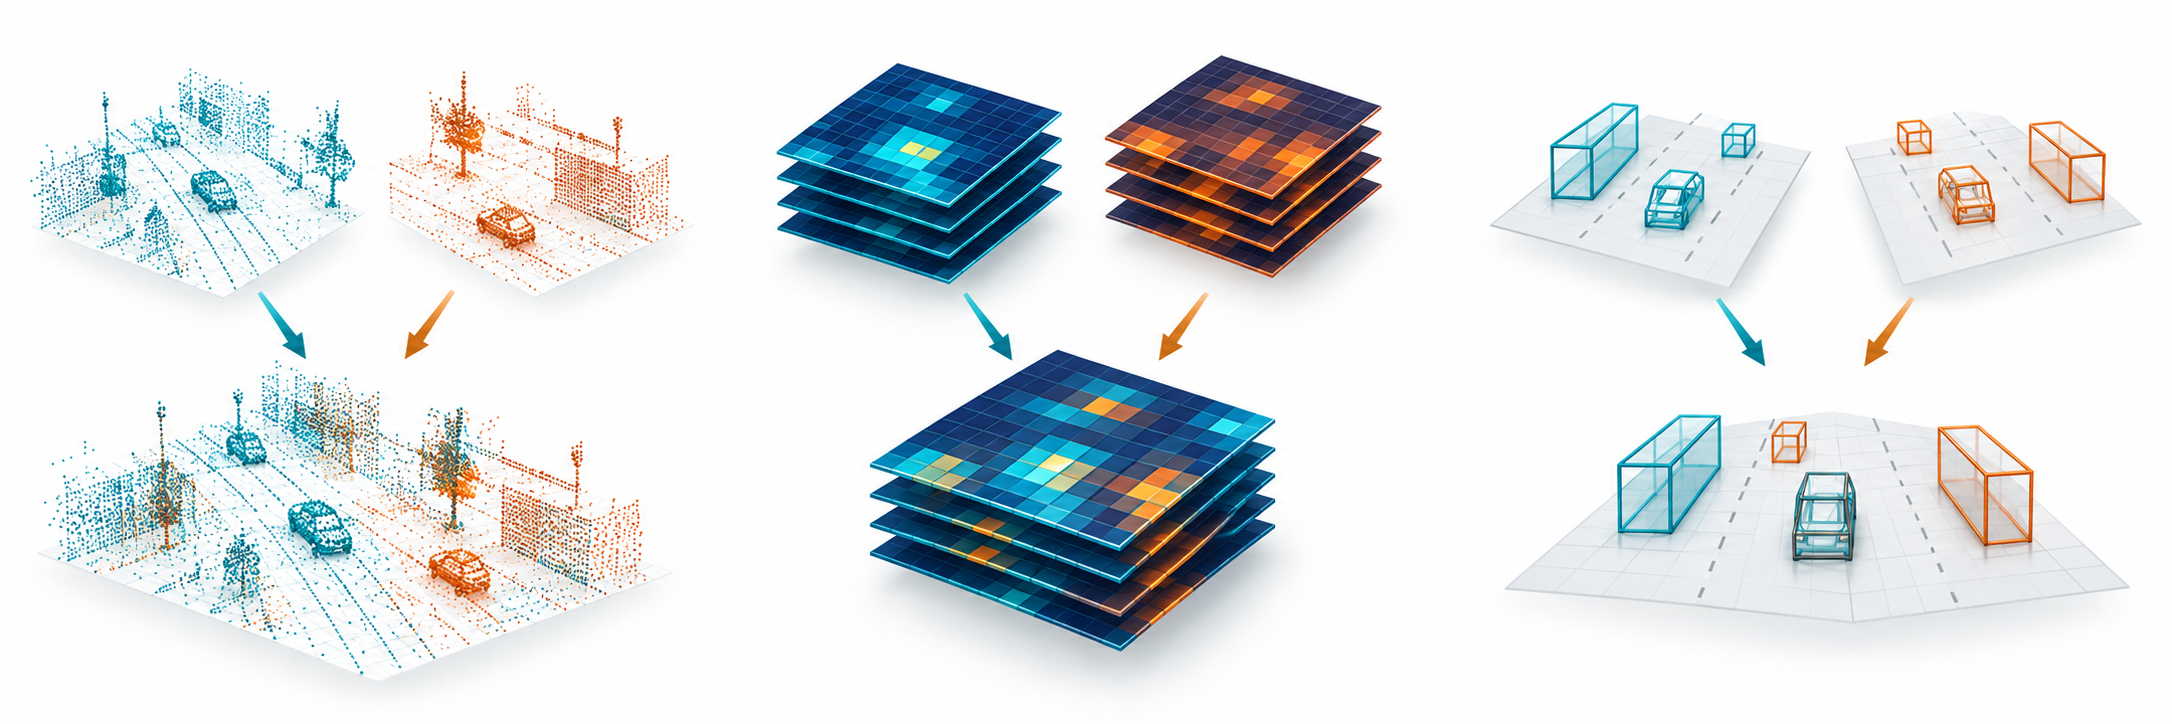
\includegraphics[width=\linewidth]{illustrations/fusion-strategies.png}
\caption[Early, intermediate, and late fusion]{The project's comparison of
raw-point, learned-feature, and detection-level combination. The colored
tensors and boxes are conceptual AI-assisted artwork.}
\label{fig:fusion-strategies}
\end{figure}

Figure~\ref{fig:fusion-strategies} makes the exchanged representation
explicit. Early fusion places information from different observers together
before encoding. Intermediate fusion lets each observer first encode its
own input. Late fusion moves collaboration after local predictions. This
ordering determines which processing is local and which information is
available when collaboration takes place.

DiscoNet uses an early-fusion teacher to guide an intermediate-fusion student
during training. The teacher has a more complete observation, while the
student receives local and shared features. Distillation encourages
correspondence between their learned representations. Only the student is
needed at inference~\cite{li2021disconet}. The evaluations in this report load
the released student checkpoint; the teacher and its distillation loss are
not run as part of the measured detection pipeline.

\begin{figure}[htbp]
\centering
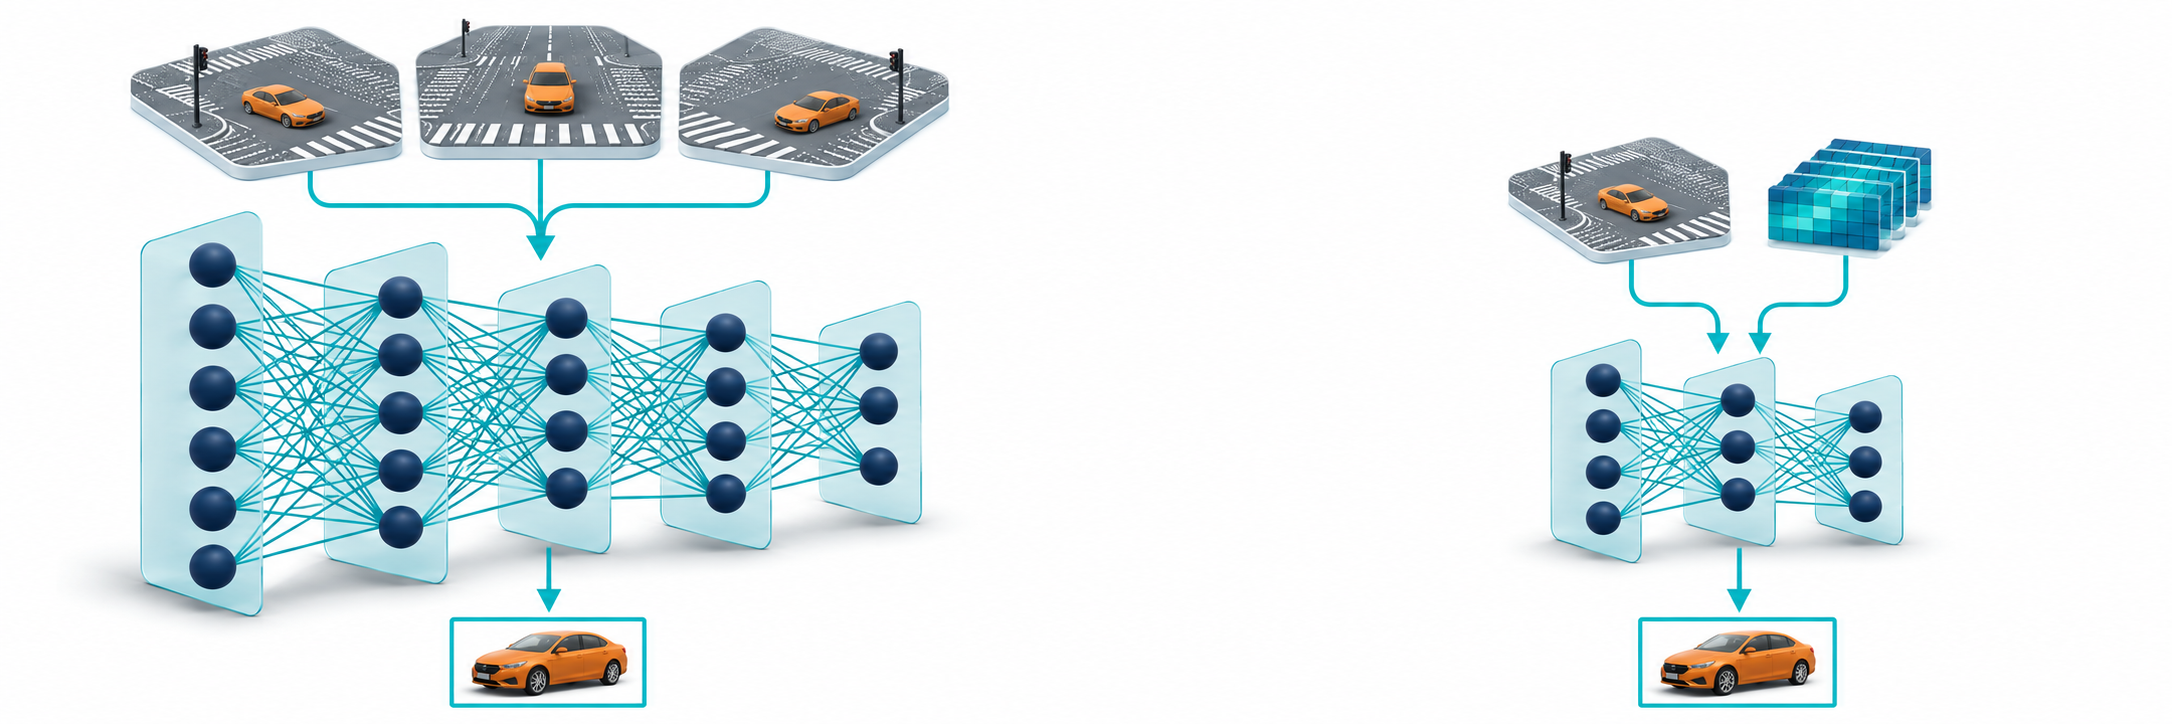
\includegraphics[width=0.92\linewidth]{illustrations/problem/problem-model-distillation-imagegen-v4.png}
\caption[Teacher guidance and the deployed student]{Project illustration
of teacher guidance and the student's detection task. Network sizes express
the teaching roles; the implemented teacher and student share the
encoder/decoder backbone.}
\label{fig:distillation}
\end{figure}

The training relationship in Figure~\ref{fig:distillation} is distinct from
the measured inference comparison. Turning sharing off restricts the same
student to its local scan. Turning sharing on provides peer features without
changing the checkpoint. The report therefore evaluates what collaboration
adds to that fixed student, rather than comparing a large teacher with a
separately trained smaller detector.

\FloatBarrier

\subsection{From LiDAR Points to Occupancy Grids}
The detector consumes the authors' prepared V2X-Sim 2.0 detection data.
CoPerception documents the preprocessing requirement and the availability of
prepared inputs~\cite{coperceptiondata}. The weekly technical material
describes the corresponding voxelization operation~\cite{recordslides}.
Invalid coordinates are rejected, and points near the sensor origin are
removed when both $-1<x<1$ and $-1<y<1$. Retained points satisfy
\[
  -32<x<32,\qquad -32<y<32,\qquad -3<z<2,
\]
with distances in meters. A binary occupancy grid uses horizontal cells of
$0.25\times0.25$ m and height bins of 0.4 m. The recorded model input has
shape $256\times256\times13$ in height--width--channels order: occupied cells
are set to one and cells without retained returns remain zero.
The reported runs start from prepared grids; raw-point preprocessing is not
part of their forward-runtime measurements.

\begin{figure}[htbp]
\centering
\begin{minipage}[c]{0.48\linewidth}
\centering
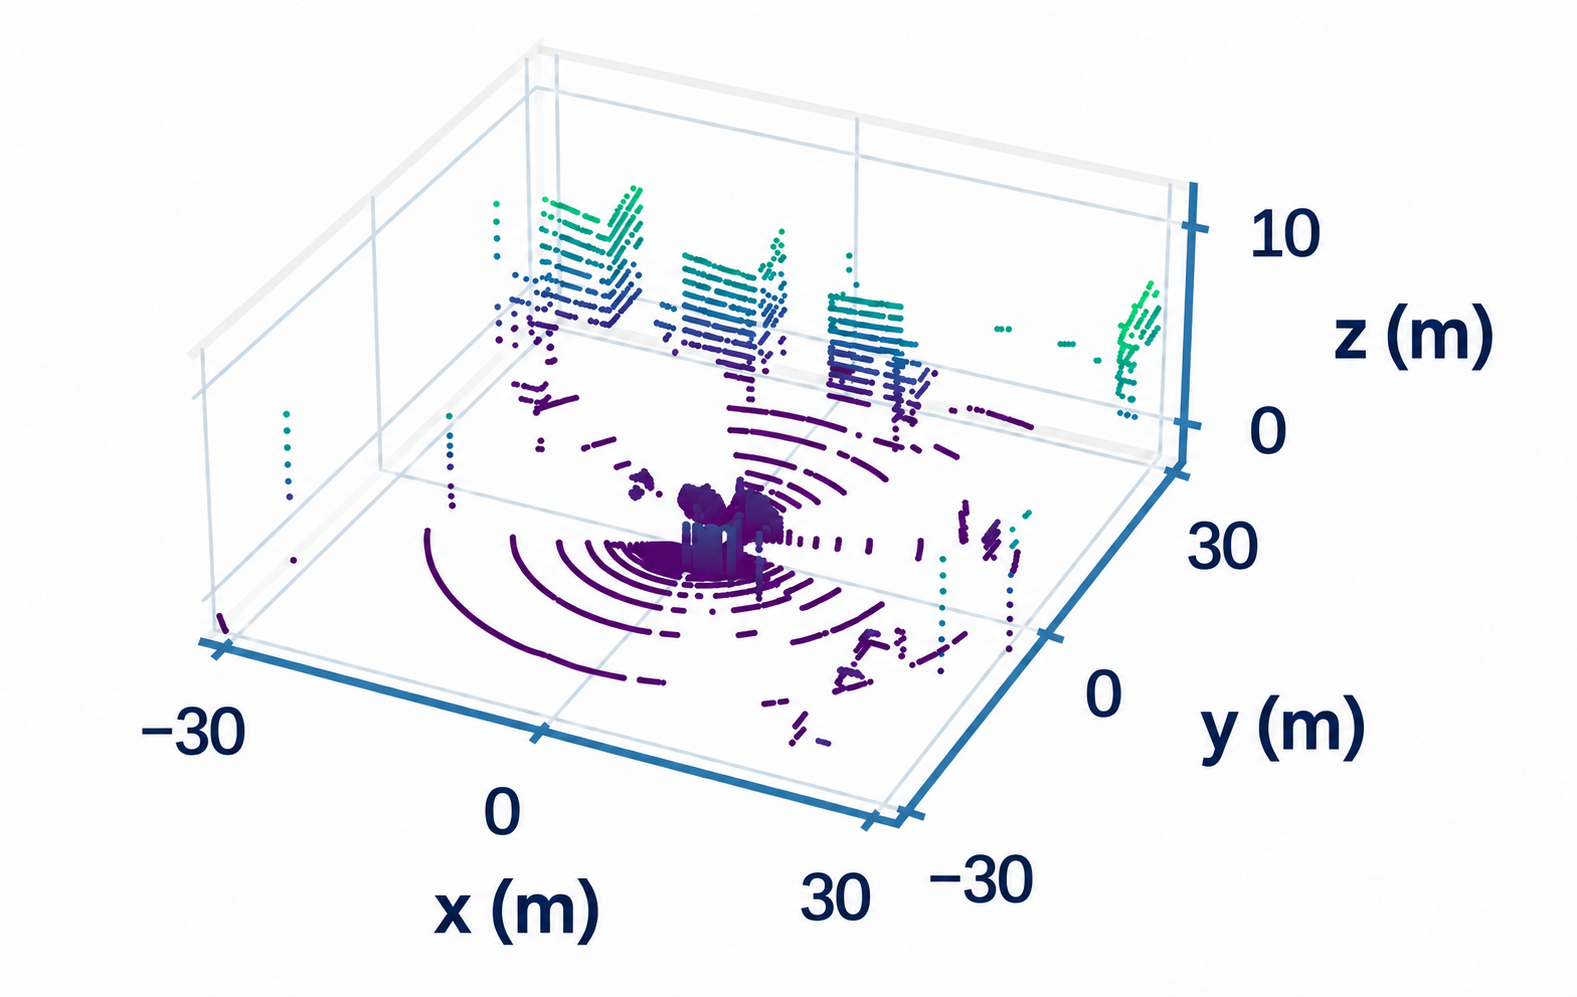
\includegraphics[width=\linewidth]{architecture/preprocessing/w44_raw_scan-imagegen-v3.png}
\small (a) A local LiDAR observation
\end{minipage}\hfill
\begin{minipage}[c]{0.48\linewidth}
\centering
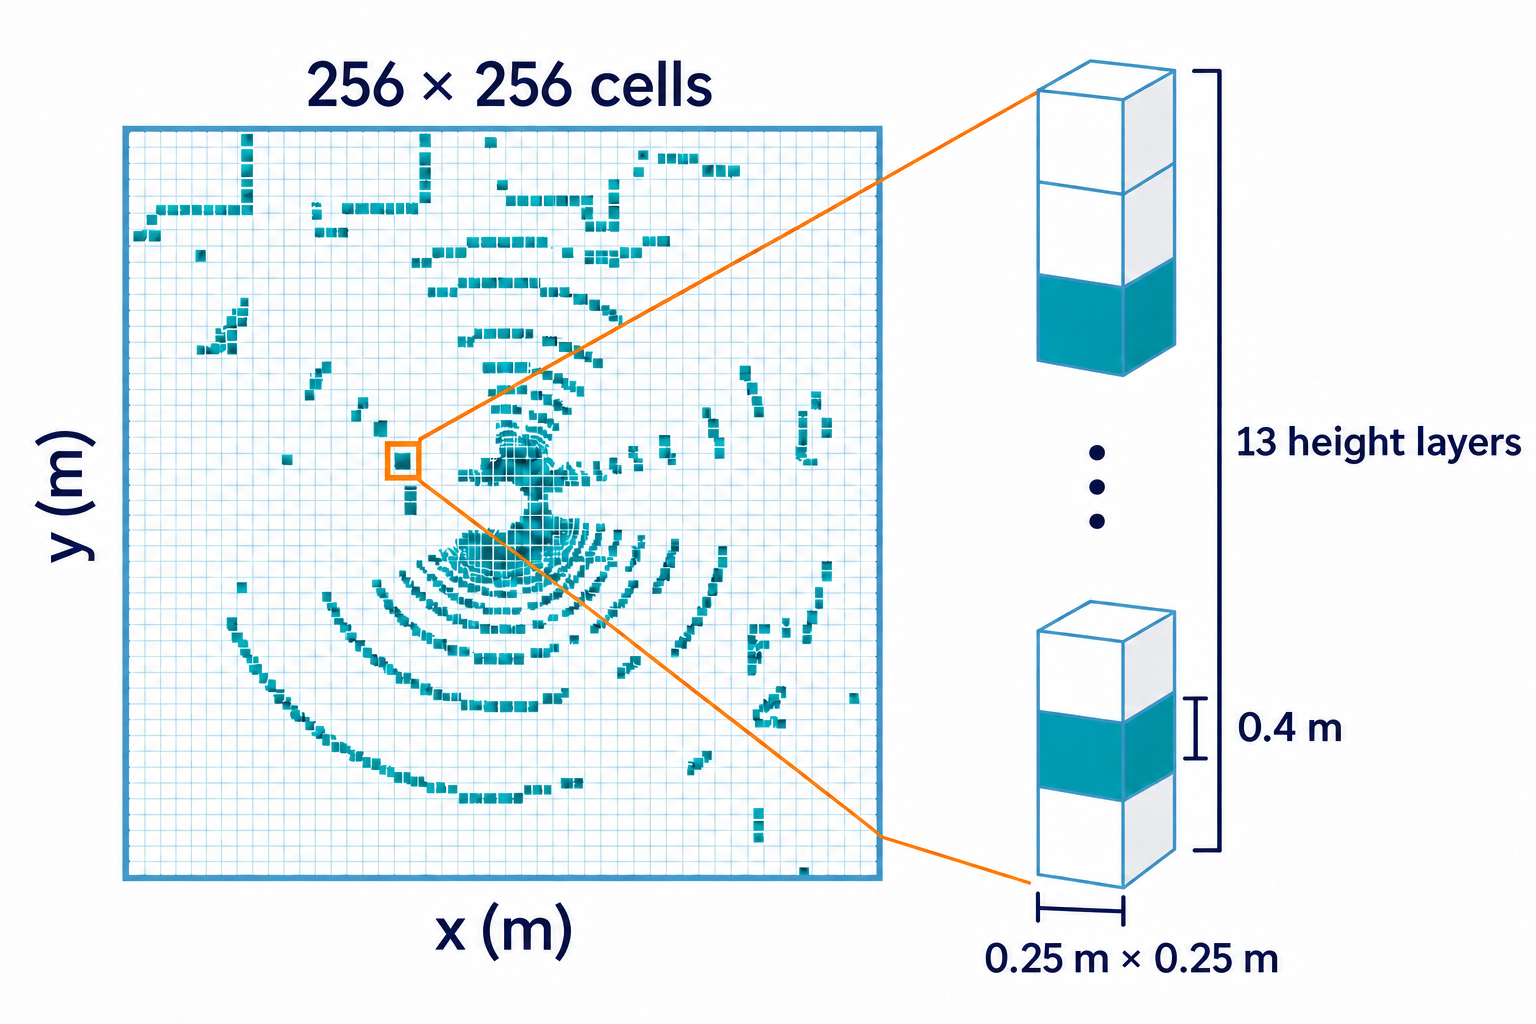
\includegraphics[width=\linewidth]{architecture/preprocessing/w44_occupancy_layers-imagegen-v3.png}
\small (b) Occupancy organized into height layers
\end{minipage}
\caption[From a local scan to occupancy height layers]{Project preprocessing
illustrations. Returns are assigned to spatial cells and height bins;
occupied cells have value one. These conceptual AI-assisted views explain
the representation rather than plotting a recorded input tensor.}
\label{fig:occupancy}
\end{figure}

The horizontal grid covers the 64-meter square around the sensor. Its
thirteen channels represent vertical occupancy bins; they are not thirteen
cameras or time steps. Figure~\ref{fig:occupancy} explains how height
information can enter a network that applies 2D spatial convolutions.
The layer stack is the channel dimension of the input feature tensor.

The diagrams use $H\times W\times C$ to make spatial size and channel
count visible. PyTorch stores 2D feature tensors in
$N\times C\times H\times W$ order. Batch and agent axes are omitted in
the illustrated shapes. These different display conventions describe the
same representation.

\FloatBarrier

\subsection{Reusable Units and the Encoder}
The architecture is assembled from a reusable 2D unit: a $3\times3$
convolution followed by batch normalization and ReLU. An Initial unit can
change channels while preserving spatial resolution; Keep preserves both;
Down uses stride two and doubles the channels. Figure~\ref{fig:encoder-units}
shows the unit and the encoder stage that composes these operations.

\begin{figure}[htbp]
\centering
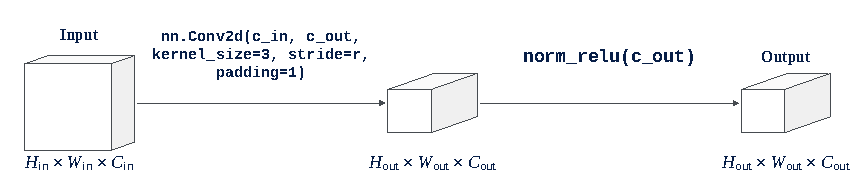
\includegraphics[width=\linewidth]{architecture/blocks/unit-2d-cubes-v4.pdf}\par
\vspace{0.6em}
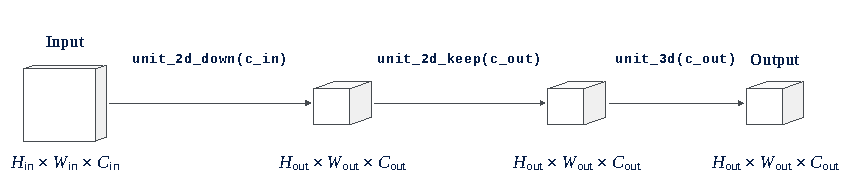
\includegraphics[width=\linewidth]{architecture/blocks/encoder-stage-cubes-v2.pdf}
\caption[The reusable 2D unit and encoder stage]{Project tensor diagrams:
the 2D unit above and its use inside an encoder stage below. The optional
pointwise 3D helper preserves the displayed spatial and channel dimensions.}
\label{fig:encoder-units}
\end{figure}

The optional 3D helper inserts a singleton depth axis, applies a
$1\times1\times1$ convolution, and flattens that axis again. Here it mixes
channels at each location rather than aggregating multiple recorded frames.
Appendix~\ref{app:implementation} contrasts this helper with a genuine
temporal convolution and gives the callable block definitions.

The encoder computes multiscale features independently for each vehicle.
Table~\ref{tab:architecture} summarizes the tensor routing shown in the
presentation. Batch and agent axes are omitted. The Stage 3 map is shared
with DiscoGraph, while the deeper Stage 4 output remains a local decoder
input. Saved encoder maps supply the decoder's skip connections.

\begin{table}[htbp]
\centering
\caption{Encoder feature shapes and routing. Tensor order is $H\times W\times C$.}
\label{tab:architecture}
\begin{ReportTable}{llL}
\ReportTableHead
\ReportTH{Stage} & \ReportTH{Output shape} & \ReportTH{Use} \\
Input & \ReportShape{256\times256\times13} & Prepared occupancy grid \\
0 & \ReportShape{256\times256\times32} & Saved for decoder Stage 8 \\
1 & \ReportShape{128\times128\times64} & Saved for decoder Stage 7 \\
2 & \ReportShape{64\times64\times128} & Saved for decoder Stage 6 \\
3 & \ReportShape{32\times32\times256} & Aligned and fused by DiscoGraph \\
4 & \ReportShape{16\times16\times512} & Local decoder input \\
\end{ReportTable}
\end{table}

\begin{figure}[htbp]
\centering
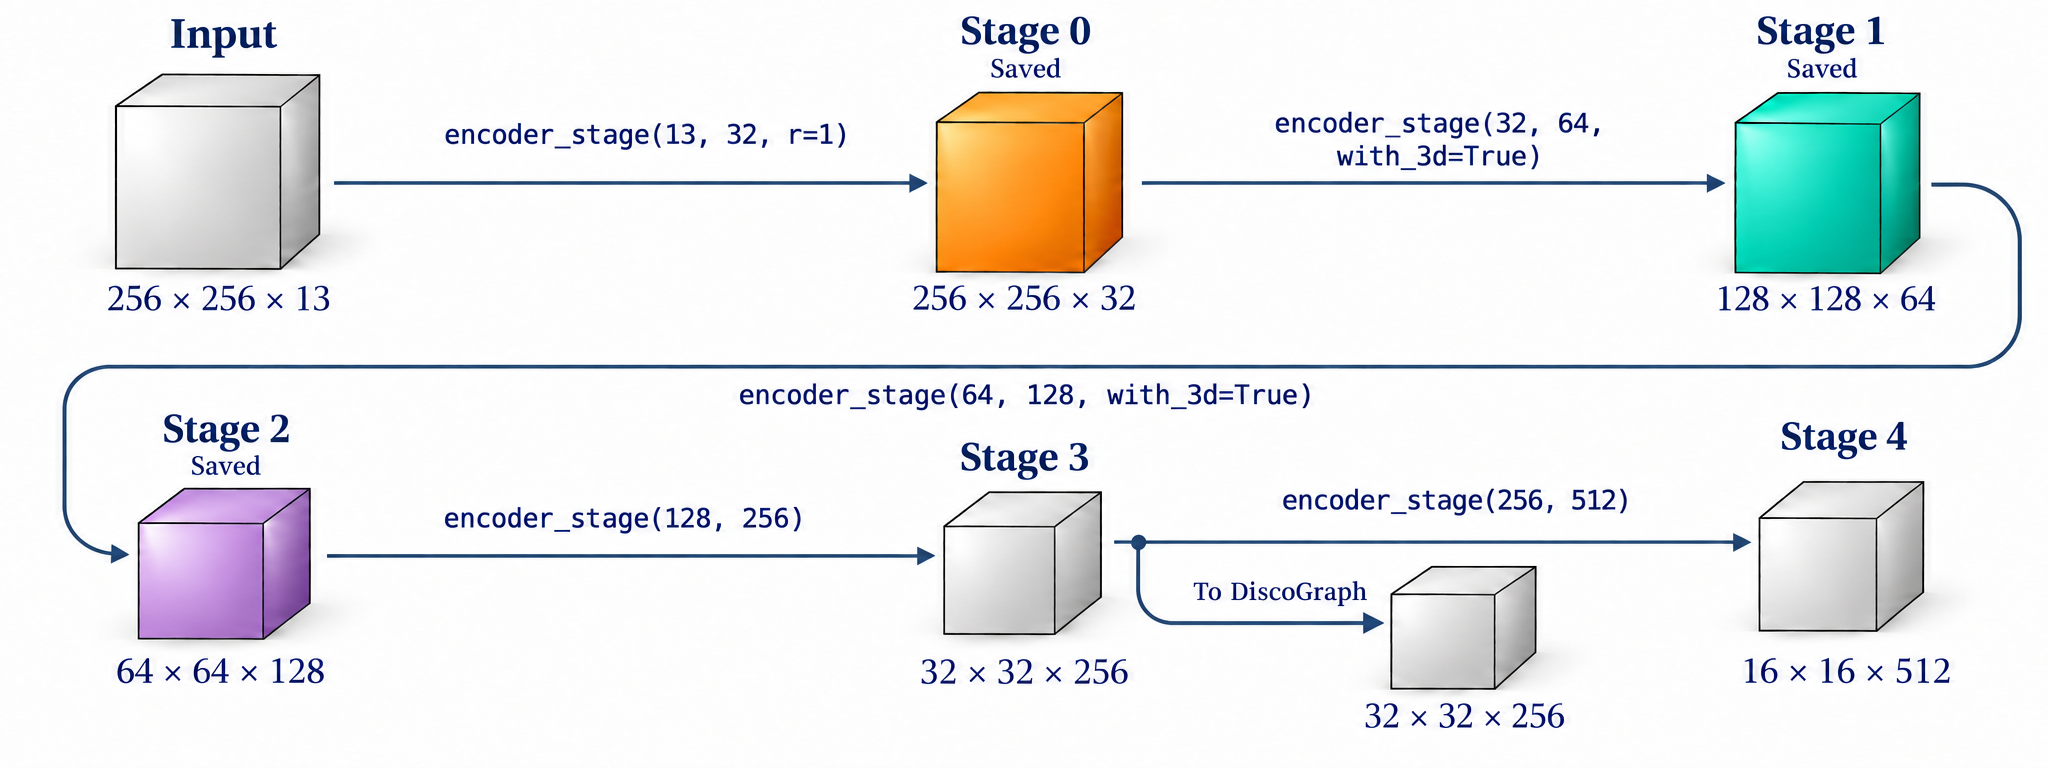
\includegraphics[width=\linewidth]{architecture/encoder/encoder-stage-pipeline-imagegen-v9.png}
\caption[Encoder tensor states and the collaboration branch]{Project encoder
pipeline illustration. Saved Stage 0--2 maps return through skip connections.
Stage 3 supplies the shared representation; Stage 4 supplies the deeper
local representation.}
\label{fig:encoder-pipeline}
\end{figure}

Spatial resolution falls as channel count increases in
Figure~\ref{fig:encoder-pipeline}. Collaboration acts on a $32\times32$
grid, with 256 channels at each location, rather than directly on the
$256\times256$ occupancy grid. The local Stage 4 path is retained alongside
this shared representation. The decoder will use both.

\FloatBarrier

\subsection{Spatial Alignment, Attention, and Fusion}
Let $F_u$ be sender $u$'s feature map and let $v$ be the receiving vehicle.
An alignment operator $\mathcal{T}_{u\to v}$ rotates and translates the
sender's map into the receiver's coordinates. It is based on their relative
poses, so the two maps describe the same physical region. In the recorded
implementation, feature resampling uses bilinear interpolation, zero padding,
and \texttt{align\_corners=False}~\cite{recordfulltest}.

\begin{figure}[htbp]
\centering
\begin{minipage}[c]{0.57\linewidth}
\centering
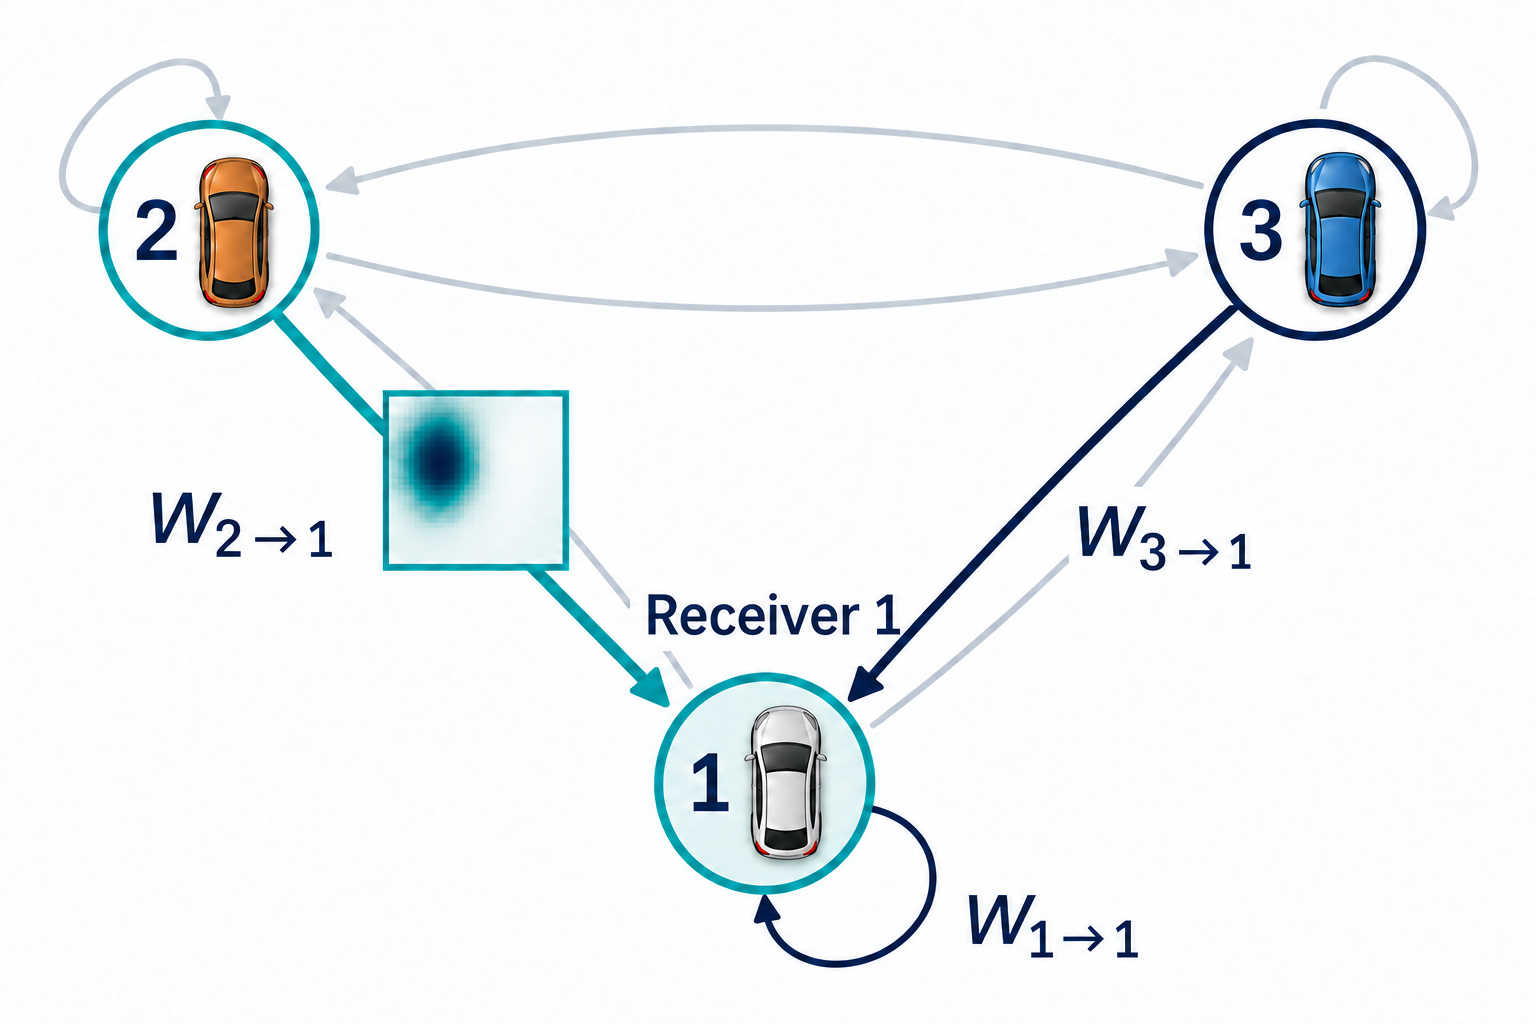
\includegraphics[width=\linewidth]{architecture/graph/discograph-three-agents-imagegen-v3.png}
\end{minipage}\hfill
\begin{minipage}[c]{0.39\linewidth}
\centering
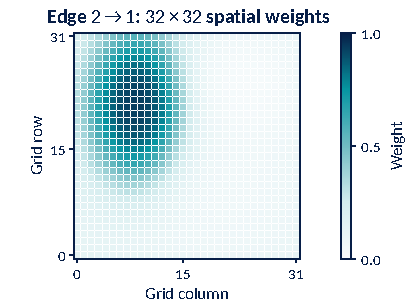
\includegraphics[width=\linewidth]{architecture/graph/discograph-three-agents-v2-spatial-map.pdf}
\end{minipage}
\caption[Directed interactions and a spatial edge-weight map]{The project's
three-agent teaching example. An edge carries a spatial weight map, so a
sender's influence can vary across the receiver's grid. Displayed weights
are synthetic examples.}
\label{fig:directed-graph}
\end{figure}

For $u\to v$, receiver $v$ defines the coordinate system. Reversing the
direction changes both the receiving grid and the feature pair being
scored. Equal array indices in two unaligned maps can refer to different
physical locations. Figure~\ref{fig:alignment} shows why corresponding
locations must be brought into agreement before their features are paired.

\begin{figure}[htbp]
\centering
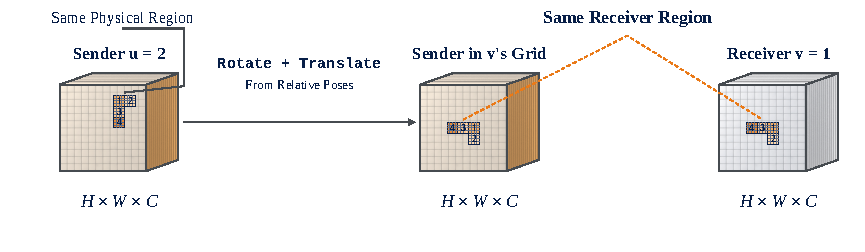
\includegraphics[width=\linewidth]{graph/discograph-step-01-alignment-v3.pdf}
\caption[Aligning sender features to the receiver's grid]{Project alignment
diagram. A pose-based transform moves the sender's representation into the
receiver's grid. The same spatial transform is applied to every channel.}
\label{fig:alignment}
\end{figure}

\begin{figure}[htbp]
\centering
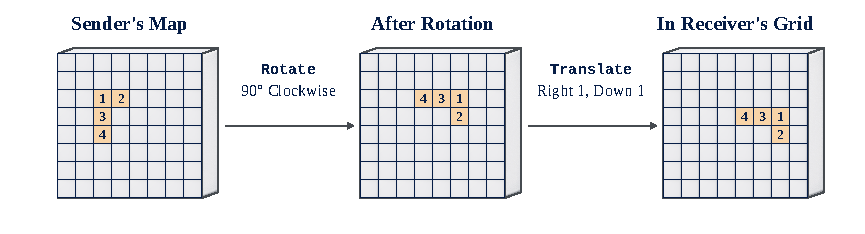
\includegraphics[width=\linewidth]{graph/discograph-rotation-translation-v3.pdf}
\caption[A worked rotation and translation on one feature channel]{The
project's $8\times8$ teaching example separates rotation from translation.
Colored cells track how a spatial pattern is relocated before fusion.}
\label{fig:rotation-translation}
\end{figure}

The small example in Figure~\ref{fig:rotation-translation} makes the
operation visible on one channel. Rotation changes the pattern's orientation;
translation changes its destination position. Feature channels remain
separate during this resampling. The sampling grid specifies where each
output cell reads the input, so output-to-input sampling uses the inverse
of a forward motion of points. The project's code example is included in
Appendix~\ref{app:implementation}.

\FloatBarrier
\subsection{Pairing Features and Computing Edge Scores}

The aligned sender features and receiver features are concatenated across
channels. A learned scoring function produces a spatial edge-score map,
\[
  s_{u\to v}(r,c)=g\!\left([F_v,\mathcal{T}_{u\to v}(F_u)]\right)_{r,c}.
\]
The implementation walkthrough reduces the paired channels through 128, 32,
and 8 intermediate channels before producing one score per spatial cell.

\begin{figure}[htbp]
\centering
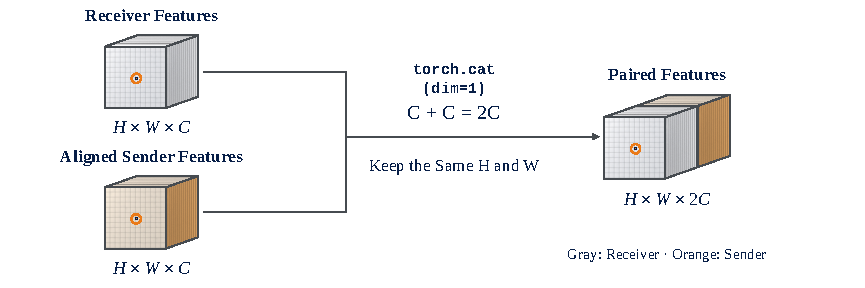
\includegraphics[width=\linewidth]{graph/discograph-step-02-pairing-v3.pdf}
\caption[Pairing receiver and aligned sender features]{Project diagram of
channel concatenation. Two 256-channel maps form a 512-channel pair at
each of the $32\times32$ collaboration locations.}
\label{fig:pairing}
\end{figure}

\begin{figure}[htbp]
\centering
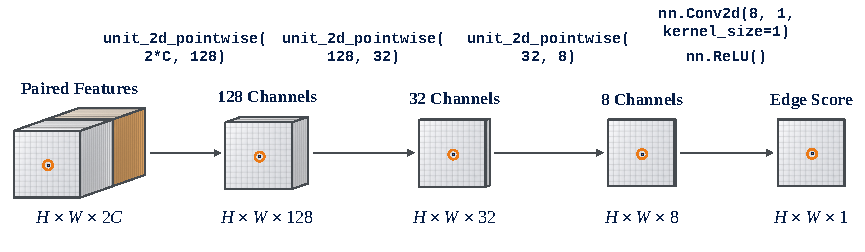
\includegraphics[width=\linewidth]{graph/discograph-step-03-scores-v4.pdf}
\caption[The edge-scoring subnetwork]{Project channel reductions from paired
features to an $H\times W\times1$ edge-score map. Spatial dimensions remain
unchanged while pointwise convolutions reduce the channel count.}
\label{fig:edge-scores}
\end{figure}

Concatenation preserves both input feature vectors rather than averaging
them. The pointwise scoring network then mixes their channels at each
location. Its final scalar describes that sender--receiver interaction
at one cell; it is distinct from the car-class confidence emitted later
by the detection head.

\FloatBarrier
\subsection{Spatial Weights and Feature Fusion}
A softmax across senders, including the receiver itself, gives
\begin{equation}
  a_{u\to v}(r,c)=
  \frac{\exp s_{u\to v}(r,c)}{\sum_{j=1}^{n}\exp s_{j\to v}(r,c)},
  \qquad \sum_{u=1}^{n}a_{u\to v}(r,c)=1.
\end{equation}

\begin{figure}[htbp]
\centering
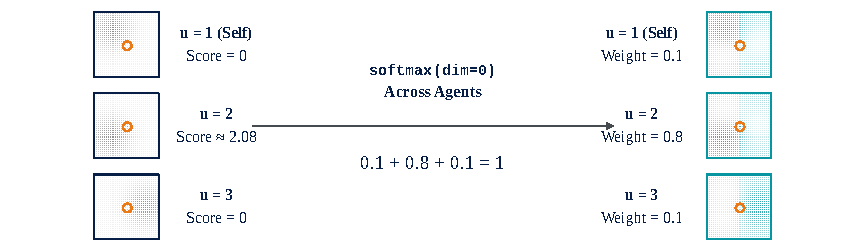
\includegraphics[width=\linewidth]{graph/discograph-step-04-softmax-v3.pdf}
\caption[Normalizing spatial weights across senders]{Project softmax
illustration. For one receiver and one cell, all contributing sender
weights sum to one. The operation is repeated across the spatial grid.}
\label{fig:spatial-softmax}
\end{figure}

Normalization acts on the sender axis, not on feature channels or on all
spatial cells together. Weights at two cells can therefore differ for the
same edge. A sender can have more influence in one region than another,
as the spatial map in Figure~\ref{fig:directed-graph} illustrates.

The fused map is
\begin{equation}
  \widetilde F_v(r,c,:)=
  \sum_{u=1}^{n}a_{u\to v}(r,c)\,
  \mathcal{T}_{u\to v}(F_u)(r,c,:).
\end{equation}
Thus, a scalar weight at a cell multiplies its entire channel vector, and
the weighted contributions are summed. The illustrated three-agent weights
in the presentation are teaching examples, not attention values measured
from these runs. Actual benchmark groups contain three to five active vehicles.

\begin{figure}[htbp]
\centering
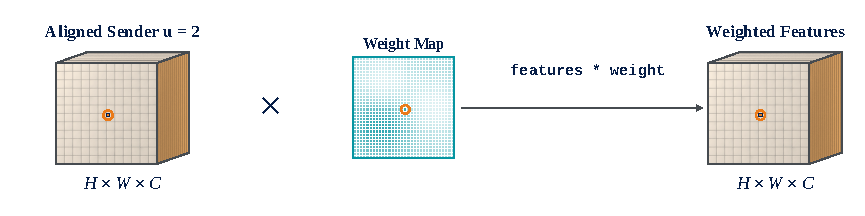
\includegraphics[width=\linewidth]{graph/discograph-step-05-weighting-v3.pdf}\par
\vspace{0.6em}
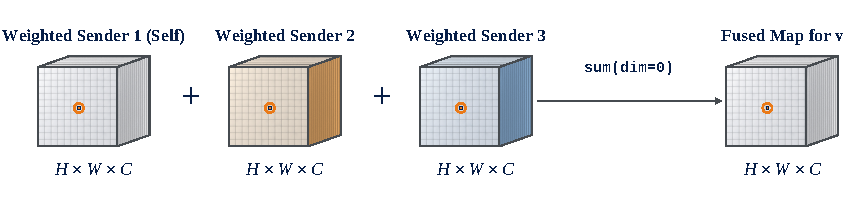
\includegraphics[width=\linewidth]{graph/discograph-step-06-fusion-v3.pdf}
\caption[Weighting contributions and summing the fused map]{Project diagrams
of the final operations. Above, a spatial scalar is broadcast over the
channel vector. Below, weighted maps, including the self contribution,
are added to form one fused map for the receiver.}
\label{fig:weighted-fusion}
\end{figure}

The fused output retains $H\times W\times C$. More senders add terms to
the sum rather than adding output channels. The self contribution keeps
the receiver's own representation in the same normalized competition as
its peer contributions. This completes one collaboration round.

\FloatBarrier
\subsection{Decoder, Skip Connections, and Detection Heads}
The first decoder stage upsamples the local Stage 4 output and concatenates
it with the fused Stage 3 map. Upsampling uses nearest-neighbor interpolation;
concatenation joins channels while matching spatial dimensions. Thus a
$16\times16\times512$ map becomes $32\times32\times512$ and is joined with
$32\times32\times256$ fused features, giving 768 channels.
Figure~\ref{fig:decoder-stage} exposes that sequence.

\begin{figure}[htbp]
\centering
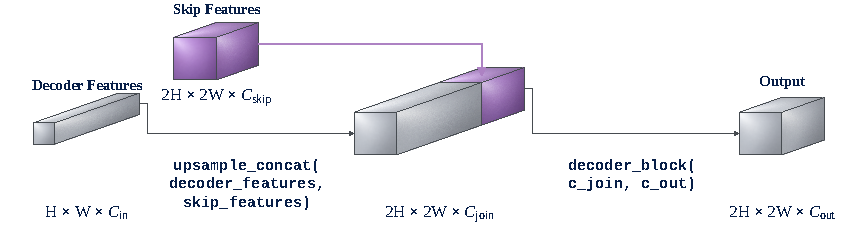
\includegraphics[width=\linewidth]{architecture/blocks/decoder-stage-cubes-v6.pdf}
\caption[Upsampling, skip concatenation, and the decoder block]{Project
decoder-stage diagram. Upsampling changes spatial size, concatenation
appends the skip channels, and the decoder block produces the next map.}
\label{fig:decoder-stage}
\end{figure}

Later stages use saved Stage 2, 1, and 0 features. Each skip already has the
target spatial resolution. The decoder block contains two 2D units with
stride one. Table~\ref{tab:decoder} records the channel arithmetic, and
Figure~\ref{fig:decoder-pipeline} shows the full route to the input grid size.

\begin{table}[htbp]
\centering
\caption{Decoder routing. All shapes use $H\times W\times C$.}
\label{tab:decoder}
\begin{ReportTable}{lLll}
\ReportTableHead
\ReportTH{Stage} & \ReportTH{Skip source} & \ReportTH{Concatenated shape} & \ReportTH{Output shape} \\
5 & Fused Stage 3 & \ReportShape{32\times32\times768} & \ReportShape{32\times32\times256} \\
6 & Saved Stage 2 & \ReportShape{64\times64\times384} & \ReportShape{64\times64\times128} \\
7 & Saved Stage 1 & \ReportShape{128\times128\times192} & \ReportShape{128\times128\times64} \\
8 & Saved Stage 0 & \ReportShape{256\times256\times96} & \ReportShape{256\times256\times32} \\
\end{ReportTable}
\end{table}

\begin{figure}[htbp]
\centering
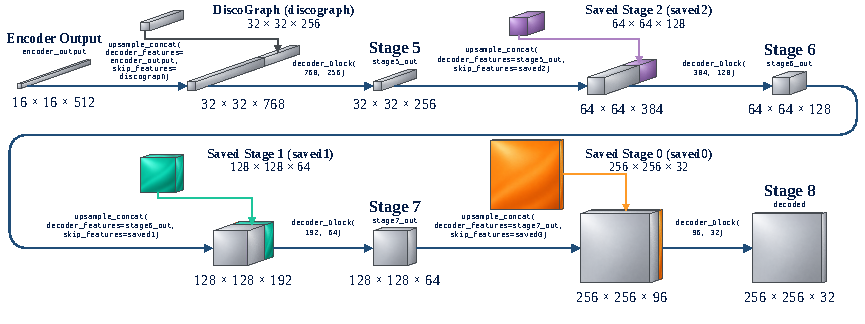
\includegraphics[width=\linewidth]{architecture/decoder/decoder-stage-pipeline-v6.pdf}
\caption[The complete decoder pipeline]{Project diagram of decoder
Stages 5--8. The first skip is the fused collaboration map; the other three
are saved local encoder maps. The output returns to $256\times256$ resolution.}
\label{fig:decoder-pipeline}
\end{figure}

The final $256\times256\times32$ map feeds classification and
box-regression heads. Classification produces background/car logits for
candidate anchors; regression produces box parameters. Decoding, confidence
filtering, and rotated NMS turn these dense outputs into the retained
detection set. Section~\ref{sec:metrics} explains its evaluation.

\subsection{Pairwise Work}
For $n$ active slots, the original complete graph evaluates $n^2$ ordered
sender--receiver pairs when self pairs are counted. There are $n(n-1)$ peer
pairs excluding self links. These are two conventions for the same graph,
not conflicting complexity claims. Pairwise collaboration contributes
quadratic work in $n$; the encoder, decoder, and heads also contribute to
the measured full-group execution time.
